\chapter{Implementação do Projeto}

\section{Bloco 0 - Conversão A/D no MSP430}
	
	\subsection{Análise de \textit{Hardware}}
	
		Antes do sinal chegar ao microcontrolador para o correto processamento do sinal de áudio, será necessário, conforme já relatamos, amostrar esse sinal através de valores corretamente quantizados. Para isso, conforme abordado na seção \ref{secao-conv-analogica-digital} deste trabalho, é necessário utilizar um Conversor Analógico Digital - ADC.
		
		O modelo do MSP 430 em questão (MSP430F5529LP) possui um ADC interno de 12 (doze) bits (ADC12). Ou seja, é possível representar em níveis de pulso até 4096 níveis. Algumas características podemos listar pois será objeto de avaliação dentro do projeto \cite{Davies2008}.
		
		\begin{itemize}
			\item Resolução de 12 bits monotônica, sem perdas de código;
			\item Velocidade nominal de até 200.000 amostras por segundo (200 Ksps), utilizando a técnica de aproximação sucessivas (SAR);
			\item Operação de com diversas referências internas de tensões: 1.5V, 2.0V, ou 2.5V com consumo típico de aproximadamente $250\mu A$ quando em operação;
			\item Canais de entrada exclusivos para sensor de temperatura interno, tensão de alimentação e tensões de referências externas;
			\item 16 memórias de conversão com controle independente de cada uma, inclusive com a capacidade de especificar o canal de entrada e referência;
			\item Fonte de \textit{clock} selecionáveis por softwares;
		\end{itemize}
	
		O coração de funcionamento desse módulo do microcontrolador consiste basicamente no seguinte:
		
			\begin{enumerate}[(i)]
				\item O processador usa dois níveis de tensões selecionáveis: $V_{R^{+}} $ e $ V_{R^{-}} $ afim de determinar o valor mínimo e máximo do conversor;
				\item Uma saída digital ($ N_{ADC} $) é setado no nível máximo ($ 4095 = 0FFFh $) quando o valor de entrada for igual ou até mesmo maior que $ V_R^+ $. De modo semelhante o valor digital ($ N_{ADC} $) será zero quando o valor de entrada for igual ou menor que $ V_{R^-} $.
				\item A equação básica da conversão é:
				
				\begin{equation}
					\label{eq-adc12-formula}
					N_{ADC} = 4095.\frac{V_{in}-V_R^-}{V_R^+ - V_R^-}
					\qquad
					V_{in}: \text{Tensão de entrada}.
				\end{equation}
				\item Em especial, o módulo ADC12\_A é configurado por dois registros de controle: o ADC12CTL0 e ADC12CTL1.
				\item  O modo de funcionamento do conversor (conversão simples ou sequência de canais) pode ser configurado pelos \textit{bits} CONSEQx (registrador ADC12CTL1);
				\item Após isso, seleciona-se o endereço inicial da memória de conversão, pelos \textit{bits} CSTARTADDx (registrador ADC12CTL1);
				\item Por fim, liga-se o conversor (\textit{bit} ADC12CTL0:ADC12ON=1) e habilitam-se as conversões (\textit{bit} ADC12CTL0:ENC=1).7
			\end{enumerate}
	
	\subsection{Requisitos de Hardware para a Tempo de Amostragem}
		
		\subsubsection{Contextualização}
		
		Um ponto importante a ser considerado, quando convertemos um sinal analógico qualquer numa sequência de valores digitais, é a precisão que estes valores representam o sinal original. 
		
		É claro que, na prática, é conveniente, para a escolha da taxa de amostragem, usar frequências muito maiores do que 2 vezes a do sinal e isso ocorre, por exemplo, quando possível.  Como é o caso  de sinais de áudio, especialmente em  CDs players,  em  que  a frequência de amostragem é de $44,1$ kbytes por segundo onde o que nos leva a 2 vezes a frequência máxima que podemos ouvir que é de 20 kHz.
		
		Por outro lado, o microcontrolador, em especial para a aplicação ora pretendida, são equipamentos alimentados por bateria e o consumo do dispositivo, nesse caso, é um requisito muito importante. Como a complexidade na obtenção das amostras aumenta em função da quantidade de amostragem que pode fazer e a potencialidade do microprocessador usado, é extremamente importante a escolha viável de uma taxa de amostragem (figura \ref{fig-taxa-de-amostragem-exemplos}) que atendam aos requisitos do projeto, ponderados com as limitações do equipamento em questão \cite{Braga2012}.
		
		\begin{figure}[!ht]
			\label{fig-taxa-de-amostragem-exemplos}
			\centering
			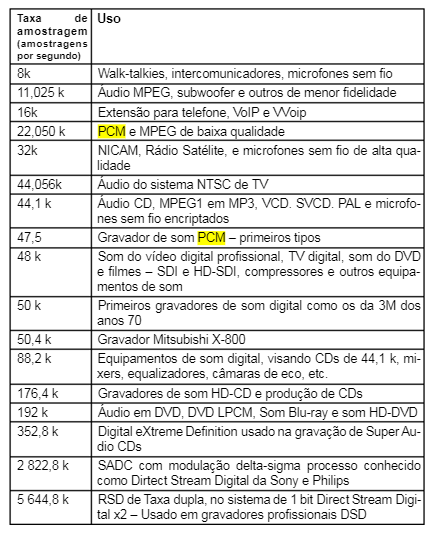
\includegraphics[scale=0.8]{./figuras/fig-exemplo-taxa-amostragem.png}
			\caption{Algumas taxas de amostragem utilizadas na prática}
		\end{figure}
	
		\subsubsection{Tempo de Amostragem do ADC12 do $\mu C$ MSP430}
			
			O conversor ADC do $\mu C$ aguarda a ocorrência de um sinal de disparo de conversão (SAMPCON) que pode ser originado de uma das quatro fontes\footnote{SHS\_1 por exemplo é proveniente da interrupção de um evento de comparação em um dos canais do timer A (saída TA1).} selecionadas pelos bits SHSx (registrador ADC12CTL1). Quando SAMCOMP = 0, todas as entradas analógicas ficam em alta impedância, caso contrário (SAMCOMP = 1), uma entrada Ax pode ser modelada como um circuito $RC$, passa baixa, durante o tempo de amostragem da conversão ($t_{sample}$).
			
			Uma equação, conforme o Guia do Usuário da Família de Microcontroladores MSP430x5xx, pode ser usada para cálculo do valor mínimo da taxa de amostragem para uma conversão de n-bits, no qual $ n $ é igual a quantidade de bits de resolução do conversor.
			
			\begin{equation}
				t_{sample} > (R_s + R_i) . \ln(2^{n+1}). C_i + 800ns
				\label{eq-circ-RC-msp430}
			\end{equation}
			
			A equação \ref{eq-circ-RC-msp430}  é oriunda de uma análise de um circuido \textit{RC} em descarregamento cuja resposta no domínio do tempo da tensão de saída é dada por:
			
			\begin{equation*}
				V_{out} = V_{in}e^{-t/{RC}}
			\end{equation*}
			
			Temos no caso, para uma quantização dos valores de tensão de entrada valores que podemos mensura-los em MSB e LSB. Considerando o caso mais simples onde a tensão de entrada estaria entre um bit 0 e 1 de uma quantização com apenas n byte ($ 2^n $ LSB`s) obtemos:
			
			\begin{equation}
				\begin{aligned}
						&\frac{V_f}{V_i} = e^{-t/{RC}}\Rightarrow \ln\left(\frac{V_f}{V_i}\right) = -\frac{t}{RC}\\
					&\ln\left(\frac{\frac{1}{2}LSB}{2^n LSB}\right) = -\frac{t}{RC}\Rightarrow \boxed{t = RC.\ln(2^{n+1})}
				\end{aligned}
			\end{equation}

			
			Por conseguinte, com SHP = 1 temos o modo de amostragem temporizada. O tempo de amostragem será determinado por um \textit{timer} interno, que é configurado de acordo com os bits SHT1x e SHT0x (registrador ADC12CTL0). Os \textit{bits} SHT1x determinam o tempo de amostragem (em ciclos de clock do conversor) para as memórias ADC12MEM8 até ADC12MEM15, tal como os \textit{bits} SHT0x determinam o tempo de amostragem para as memórias ADC12MEM0 até ADC12MEM7.
			
			Em suma, calculado o tempo de amostragem 
			
\section{Bloco 1 - Projetando um Filtro FIR}
	\subsection{Para o código Experimental do MATLAB}
		
		Para o código que foi elaborado com o objetivo de análise do efeito \textit{shimmer} e suas limitações em termos da discretização do sinal no domínio do tempo na perspectiva de síntese e análise do sinal.
		
		Nesse caso, o filtro escolhido foi um filtro FIR-passa baixa cuja frequência de corte do projeto foi no valor de 2kHz. Tendo esse filtro utilizado a quantidade de 51 \textit{Taps} (tamanho da janela), cujo janelamento foi feito com a janela \textit{Blackman} (equação \ref{eq-proj-fir1}), cujos benefícios já foram explicados anteriormente.
		
		\begin{equation}
			J = 0.42 + 0.5\cos((2\pi t)/Ntaps) + 0.08\cos((4\pi t)/Ntaps);
			\label{eq-proj-fir1}
		\end{equation}
		
		Com isso bastou-se multiplicar a resposta da janela com um filtro ideal passa-baixa ideal (equação \ref{eq-proj-fir2}), cuja frequência normalizada vale $W_1 = \pi.\left(\frac{2000}{44100/2}\right)$:
		
		\begin{equation}
			h= (W1/pi).sinc((W1/pi)t);
			\label{eq-proj-fir2}
		\end{equation}
		
		Após a multiplicação basta agora efetuar a operação de convolução com o sinal original de 12 bits resultando num sinal de 12 bits filtrado em $ 2kHz $.
	
	\subsection{Para o projeto do $ \mu $C}
		
		Com respeito ao projeto do microcontrolador, sabe-se que há uma limitação do próprio hardware em trabalhar com valores em ponto flutuante. Nesse sentido a utilização do software WinFilter foi de suma importância pois ele fornece um vetor de coeficientes do filtro FIR correpondente de acordo com os parâmetros do projeto, algo extremamente prático.
		
		Além disso ele fornece uma pequena função que já calcula a convolução das amostras do filtro, no entanto a implementação é ineficiente devido que para cada nova amostra que chega do sinal, ele desloca todas as amostras para então realocar espaço para amostra que chega:
		
		\begin{lstlisting}[caption={Código Gerado no WinFilter para um filtro FIR},label={lst:cod-winfilter01},language=C]
			//shift the old samples
			for(n=Ntap-1; n>0; n--)
			x[n] = x[n-1];
			
			//Calculate the new output
			x[0] = NewSample;
			for(n=0; n<Ntap; n++)
			y += FIRCoef[n] * x[n];
			return y / DCgain;
		\end{lstlisting}
		
		Nesse caso, há um desperdício de processamento o qual é solucionado com a implementação de um ponteiro que sempre sobrescreva as amostras antigas assim que ele chegar no fim do vetor (\textit{buffer}) predeterminado para carregar as amostras vindas do conversor A/D. Essa forma é conhecida como \textit{ring-buffer} (buffer em anel - figura \ref{fig-ringbuffer}).
		
		\begin{figure}[!ht]
			\centering
			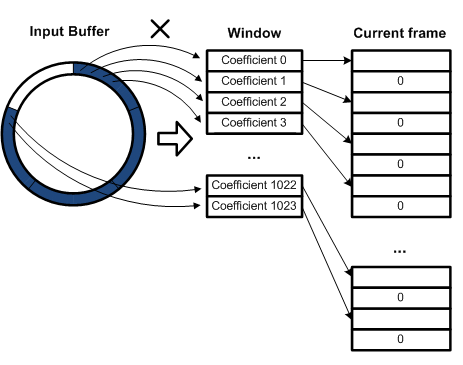
\includegraphics[scale=0.5]{./figuras/ringbuffer.png}
			\caption{Uma pequena ilustração como funciona um \textit{ring-buffer}}
			\label{fig-ringbuffer}
		\end{figure}
		
		Depois de superada essa parte do processamento a convolução das amostras se dá na segunda parte do código \ref{lst:cod-winfilter01}.
		
				
\section{Bloco 2 - Implementando o \textit{Pitch-Shifter}}

	\subsection{Análise do Algoritmo}
		\subsubsection{Conceito Preliminar - O que é necessário implementar?}
			
			Nós sabemos que o objetivo agora nesse bloco é alterar a frequência do sinal sem alterar sua duração. Uma forma que aparentemente funcionaria é que: se gravarmos um som e então faz-lo tocar duas vezes mais rápido, então a frequência desse sinal seria dobrada e então deslocada a frente 1 oitava. Isso está correto, no entanto o sinal é \textbf{duas vezes também mais curto}.
			
			A maneira de fazer isso corretamente é pegar o som gravado, dobra-lo de tamanho sem afetar sua frequência natural e então toca-lo duas vezes mais rápido, logo todas as frequências dobrariam de valor e então, devidamente deslocadas, bem como a duração do sinal nesse caso estaria mantida conforme o som original. O algoritmo do MATLAB, nesse caso se baseia nesse princípio. O que será explicado na próxima seção.
			
		\subsubsection{Implementação do Algoritmo}
			\paragraph{Visão Geral}		
				
				Um fato de escala já visto na seção \ref{introd-pitch-shift} mostra que um fator de escala é definido como um fator usado para expandir ou comprimir o espectro para ajustar as frequências do sinal de modo que esse deslocamento seja corretamente ajustado. Uma vez feito isso, nós poderemos reconstruir o sinal e voltar a sua duração inicial com o efeito \textit{pitch-shifting} realizado.
				
				De fato, se queremos deslocar o sinal um semitom, será preciso utilizar um fator de escala igual a $2^{1/12}$ o qual corresponde a $1.0594$ (figura \ref{fig-pitch-shifter-exem01}). Isto é, precisamos esticar o sinal sem alterar seu espectro de frequência a qual a duração é agora multiplicado por $1.0594$. Uma vez feito isso, somente será preciso tocar o sinal 1.0594 vezes mais rápido \cite{Demers2009}.
				
				\begin{figure}[!ht]
					\centering
					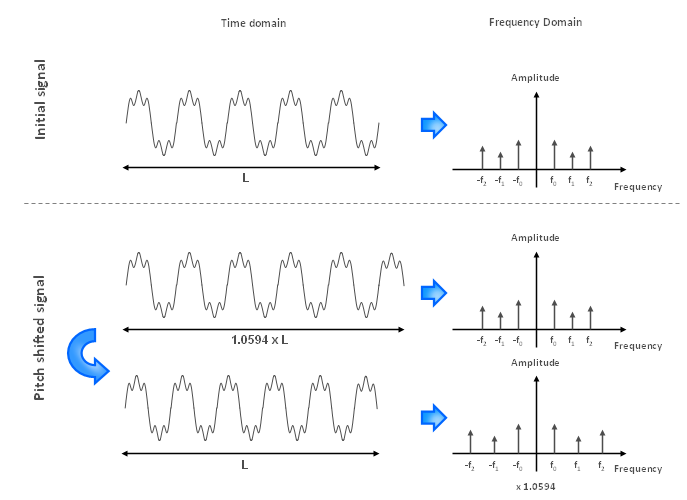
\includegraphics[scale=0.5]{./figuras/pitch-shifter-exem1.PNG}
					\caption{Exemplo de arbodagem do \textit{pitch-shifter} - premissa básica para o efeito \textit{shimmer}.}
					\label{fig-pitch-shifter-exem01}
				\end{figure}
				
				Uma das etapas de implementação do algoritmo é a separação do sinal original em uma grande quantidade de \textit{frames} (pedaços). Esses \textit{frames} (figura \ref{fig-pitch-shifter-exem02}) são obtidos do sinal original os quais são "sobrepostos" uns com os outros por um fator de 75\% de sobreposição. Esse \textit{frames} estarão então espaçados dependendo se o sinal, no processamento, será esticado ou comprimido no tempo na sua saída.
				
				\begin{figure}[!ht]
					\centering
					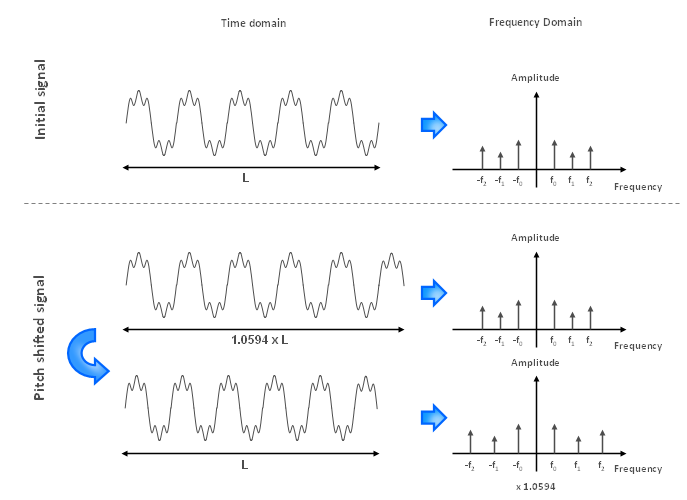
\includegraphics[scale=0.5]{./figuras/pitch-shifter-exem1.PNG}
					\caption{Expansão e compressão do sinal \textit{frame} por \textit{frame}.}
					\label{fig-pitch-shifter-exem02}
				\end{figure}
				
				No entanto, a medida que essa operação é realizada teremos um problema muito comum, pois o espaço entre os \textit{frames} são feitos em determinados trechos do sinal inadvertidamente. Nesse caso, é criado diversas descontinuidades. Isso é mostrado na figura \ref{fig-pitch-shifter-exem03} que mostra os espaços entre os frames é dado como tamanho $ x $ e torna-lo tamanho $ y $.
				
				\begin{figure}[!ht]
					\centering
					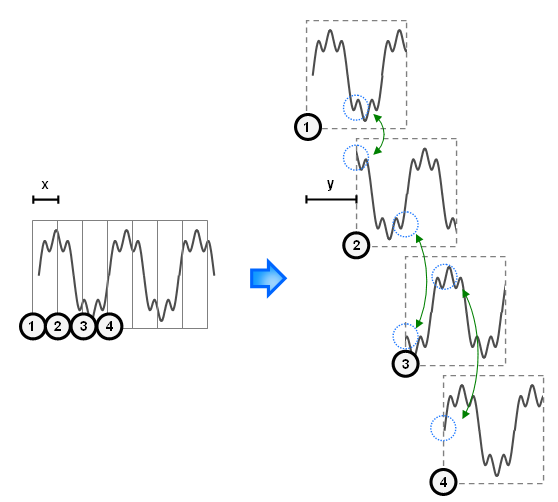
\includegraphics[scale=0.5]{./figuras/pitch-descont.PNG}
					\caption{Sinal tornando-se descontínuo quando submetido ao processo de expansão ou compressão no tempo.}
					\label{fig-pitch-shifter-exem03}
				\end{figure} 
				
				Esse procedimento produz "defeitos" no som (espaços indesejados) que são perceptíveis ao ouvido humano. Desse modo é preciso de alguma forma fazer essa descontinuidade desaparecer. Por conta disso precisamos de uma técnica de processamento denominada de \textit{phase vocoder}.
				
			\paragraph{\textit{Phase Vocoder}}
				\label{parafrafo-phase-vocoder}
				
				O \textit{phase vocoder} é uma variação na Transformada Rápida de Fourier (FFT) que usa informações de fase para melhorar as estimativas de frequência \cite{Sethares}. É ideal para uso em aplicações como o alongamento  ou a compressão de tempo de áudio, embora existam vários outros efeitos especiais que podem ser implementados usando a estratégia de \textit{phase vocoder}.
				
				Além disso, o \textit{phase vocoder} é geralmente apresentado como uma solução de alta qualidade para a modificação da escala de tempo (ou frequências), o pitch-shift é geralmente implementado como uma combinação de escala de tempo e conversão da taxa de amostragem \cite{Laroche1999}.
				
				A figura \ref{fig-phase-vocoder-introd} mostra como um algoritmo phase vocoder funciona tanto de maneira geral (figura \ref{fig-phase-vocoder-introd-B}), tal como com a implementação do algoritmo escrito em MATLAB (figura \ref{fig-phase-vocoder-introd-A}). Ele basicamente consiste em 3 (três) estágios: \underline{análise}, \underline{processamento} e \underline{síntese} \cite{Portnoff1976}. 
				
				\begin{figure}[ht!]
					\centering
					\subfigure[Ilustração Específica das Etapas do algoritmo do \textit{phase-vocoder}]{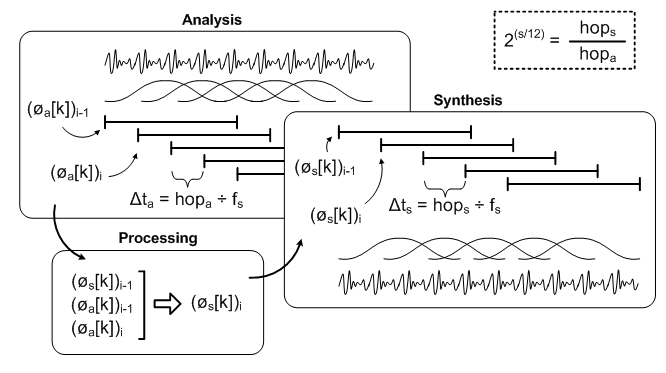
\includegraphics[scale=0.5]{./figuras/phase-vocoder-01.PNG}
					\label{fig-phase-vocoder-introd-A}
					}
					\qquad
					\subfigure[Ilustração Geral da Etapa do algoritmo \textit{phase-vocoder}]{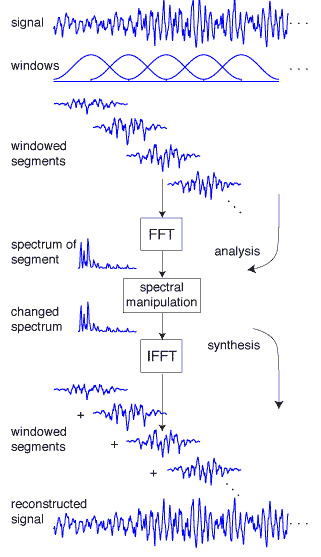
\includegraphics[scale=0.5]{./figuras/phase-vocoder-04.PNG}
					\label{fig-phase-vocoder-introd-B}
					}
					\caption{Etapas do algoritmo do \textit{phase-vocoder}}
					\label{fig-phase-vocoder-introd}
				\end{figure}
					
				\subparagraph{Análise:}
				
					Como já mencionado nesse trabalho na seção \ref{secao-janelamento} que um janelamento refere-se a falar de um pequeno \textit{frame} de um sinal infinitamente maior (se considerarmos apenas 1 pequena janela comparado a todo o sinal amostrado). O processamento dessa janela no espectro do sinal pode ser minimizada. Em outras palavras, para reduzir o efeito de janelamento do sinal na sua representação no domínio da frequência, é utilizado uma janela do tipo \textit{Hanning} ou \textit{Blackman} de tamanho $ N $. O porquê disso? Bem, de acordo coma  figura \ref{fig-phase-vocoder01}, uma multiplicação de uma janela retangular no domínio do tempo com o sinal é equivalente a uma convolução de no domínio da frequência. Desse moro a janela retangular possui mais energia nos lóbulos laterais em comparação aos demais janelamentos, enquanto a janela \textit{Hanning} ou \textit{Blackman} tem um foco de concentração de sua energia espectral no seu lóbulo principal, ou seja, perto do nível DC do sinal.
					
					\begin{figure}[!ht]
						\centering
						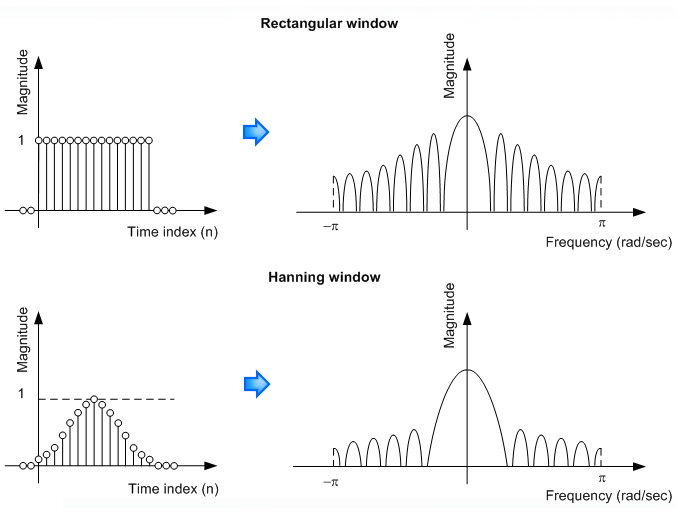
\includegraphics[scale=0.5]{./figuras/phase-vocoder-02.PNG}
						\caption{Janelamentos}
						\label{fig-phase-vocoder01}
					\end{figure}
					
					Esse frame é, o qual é formado por $ N $ amostras, é então transformado através de uma Transformada Rápida de Fourier - \textit{Fast Fourier Transform} (FFT) conforme a equação \ref{eq-phase-vocoder01}
					
					\begin{equation}
						(X_a[k])_i = \sum_{n=0}^{N-1}x[n+i.(hop_a)]w[n]e^{-j(\frac{2\pi kn}{N})}
						\qquad k = 0,1,2,...,N_1
						\label{eq-phase-vocoder01}
					\end{equation}
					
					Na equação acima, $ x[n] $ é a amostra do sinal, $ w[n] $ representa o janelamento $ Hanning $ ou $ BlackMan $ e $ (X_a[k])_i $ representa o espectro discreto do \textit{frame} $ i $. Afim de aumentar a resolução do espectro, as janelas são sobrepostas com um fator de $ 75\% $. O número de amostras entre duas sucessivas janelas é referenciado pelo "número de saltos" entre cada janela -  termo \textit{hop size} ($ hop_a $) e é igual a $ \frac{N}{4} $ de uma sobreposição de $ 75\% $.
				
				
				\subparagraph{Processamento:}
				
					Já é sabido que aplicando a FFT num sinal de tamanho $ N $ resulta em $ N $ segmentos espectrais que começam do valor $ 0 $ até o valor $ \frac{(N-1)}{N}f_s $ com um intervalo de $ \frac{f_s}{N} $, onde $ f_s $ é a nossa frequência de amostragem do sinal. Em termos de módulo, um sinal que possua uma frequência intermediária entre os dois segmentos espectrais terá seu valor não computado e a energia contida nessa frequência, distribuída entre os dois segmentos vizinhos. A informação de fase do sinal é usado para melhorar a acurácia do estimado dessas frequências entre cada segmento espectral. A figura \ref{fig-phase-vocoder02} mostra duas ondas senoidais com uma pequena diferença em valores de frequência. Conforme o método, os frames do sinal são divididos dentro das $ N $ amostras. As janelas nesse caso não estão sobrepostas para facilitar a explicação. O primeiro sinal tem a frequência de $ \frac{f_s}{N} $ e ela, de fato, cai exatamente na primeira frequência do primeiro segmento espectral. A segunda senoide, por sua vez, tem uma frequência levemente maior que o primeiro sinal. Observe que a amostra não está centrado no primeiro segmento, embora sua energia esteja principalmente no dentro dele.
				
					\begin{figure}[ht!]
						\centering
						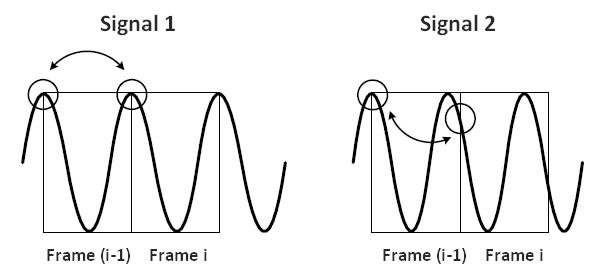
\includegraphics[scale=0.5]{./figuras/phase-vocoder-03.PNG}
						\caption{Ondas senoidais com pequena diferença na frequência e fase.}
						\label{fig-phase-vocoder02}
					\end{figure}
				
					A informação de fase de dois \textit{frames} sucessivos é significativamente relevante. Pois o primeiro sinal, não há diferença de fases entre os dois frames. Por outro lado, para o segundo sinal, a fase do primeiro segmento é maior que zero. Isso implica que a componente do sinal que correspondente para este segmento é maior que a frequência desse segmento. A diferença de fase entre dois frames é referenciado no código como \textit{phase-shift} $ (\Delta\phi_a[k])_i $ no intervalo de $ -\pi $ a $ \pi $. Sem a sobreposição, a frequência real $ (\omega_{true}[k])_i $ pode ser obtida de um deslocamento de fase $ (\Delta\phi_a[k])_i $ e um intervalo de tempo $ \Delta t_a $ entre dois \textit{frames} conforme visto na equação \ref{eq-phase-vocoder02}. O intervalo de tempo $ \Delta t_a $ é o número de saltos $hop_a$, já visto no págrafo de análise, dividido pela frequência de amostragem $ f_s $.
					
					\begin{equation}
						\label{eq-phase-vocoder02}
						(\omega_{true}[k])_i = \frac{(\Delta\phi_a[k])_i}{\Delta t_a}
					\end{equation}
					
					A equação supracitada é menos complexa pois trata-se de um sinal não sobreposto. No caso mais complexo, o desvio de frequência para o primeiro segmento é calculado e então sobreposto. Essa quantidade é adicionada ao segmento de frequência para obter a real frequência daquele componente dentro do \textit{frame}. As equações \ref{eq-desvio-frequencia}, \ref{eq-wrapped-frequency} e \ref{eq-true-frequency} ilustram esse procedimento. A variável $(\phi_a[k])_{i-1}$ e $(\phi_a[k])_i$ correspondem a fase do frame anterior e o frame presente respectivamente. Também, $ \omega_{bin}[k] $ corresponde a frequência do segmento, $ (\Delta\omega[k])_i $ o desvio de frequência e $ (\Delta\omega_{wrapped}[k])_i $ corresponde o desvio de frequência sobreposta (\textit{wrap-frequency}).
					
					\begin{equation}
						\label{eq-desvio-frequencia}
						(\Delta\omega[k])_i = \frac{(\phi_a[k])_i - (\phi_a[k])_{i-1}}{\Delta t_a} - \omega_{bin}[k]
					\end{equation}
					
					\begin{equation}
						\label{eq-wrapped-frequency}
						(\Delta\omega_{wrapped}[k])_i = \mod[((\Delta\omega[k])_i+\pi),2\pi]-\pi
					\end{equation}
					
					\begin{equation}
						\label{eq-true-frequency}
						(\omega_{true}[k])_i = \omega_{bin}[k] + (\Delta\omega_{wrapped}[k])_i
					\end{equation}
					
					A nova fase de cada fragmento pode ser então calculada adicionando a fase deslocada requerida para assim evitar-se a descontinuidade dos segmentos. Isso é feito multiplicando a frequência real com o intervalo de tempo do estágio de síntese, conforme mostrado na equação \ref{eq-ajuste-da-fase}:
					
					\begin{equation}
						\label{eq-ajuste-da-fase}
						(\phi_s[k])_i = (\phi_s[k])_{i-1} + \Delta_{t_s} . (\omega_{true}[k])_i
					\end{equation}
					
					A fase do frame anterior, por síntese, já é conhecida desde que ela á foi calculada pelo algoritmo de recursividade. Por fim, o novo espectro é então obtido conforme a equação \ref{eq-amplitude-fase-phase-vocoder}:
					
					\begin{equation}
						\label{eq-amplitude-fase-phase-vocoder}
						|(X_s[k])_i| = |(X_a[k])_i|
						\qquad
						\angle (X_s[k])_i = (\phi_s[k])_i
					\end{equation}
					
				\subparagraph{Síntese:}
					
					Agora, como já gerenciado o ajuste de fase no domínio da frequência para as sequências de frames, será preciso agora retornar ao domínio do tempo. Para isso aplicamos a Transformada Inversa Discreta de Fouriter (IDFT) para cada frame do espectro. O resultado é então um janelamento com a janela apropriada (\textit{Hanning} ou \textit{Blackman}) obtendo $ q_i[n] $. O janelamento é usado dessa vez para suavizar o sinal. Esse processo é descrito na equação \ref{eq-sintese-phase-vocoder}:
					
					\begin{equation}
						\label{eq-sintese-phase-vocoder}
						q_i[n] = \left(\frac{1}{N}\sum_{k=0}^{N-1}(X_s[k])_i e^{-j\frac{2\pi k n}{N}}\right)w[n]
						\qquad
						n = 0,1,2,...,N-1
					\end{equation}
					
					Cada \textit{frame} é estão sobreposto conforme mostra a equação \ref{eq-overlap-sintese}. A variável $ L $ corresponde ao número de \textit{frames} e $ u[n] $ representa a função degrau unitário.
					
					\begin{equation}
						\label{eq-overlap-sintese}
						y[n] = \sum_{i=0}^{L-1} q_i[n-i.hop_s]\{ u[n-i.hop_s]-u[n-i.hop_s-L]\} 
					\end{equation}
			
			\subsubsection{Reamostragem do Sinal}
				
				Agora que temos o nosso sinal sem descontinuidades podemos agora estica-lo ou comprimi-lo no tempo e suas componentes de frequências não serão alteradas. Agora, podemos re-amostrar o sinal 	e volta-lo para a duração inicial e então deslocar a sua frequência. Supondo que dado uma taxa de amostragem queremos dobrar a frequência - 1pitch de 1 oitava. A maneira mais fácil de fazer é escolher apenas uma amostra de duas e produzir o resultado. Isso é fácil, porque quando dobramos a frequência, lidamos com um fator de escala que é um número inteiro. Para fatores de escala não inteiros (1 semitom por exemplo - 1.0594) é usado uma interpolação linear para aproximar a amostra que deveria estar naquele local.
				
				\begin{figure}[!ht]
					\centering
					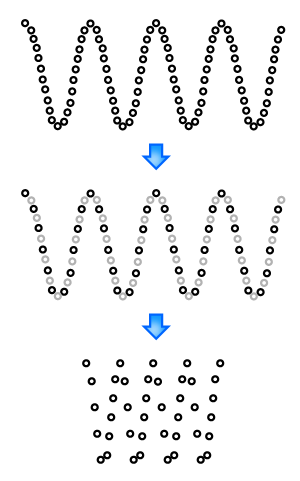
\includegraphics[scale=0.7]{./figuras/phase-vocoder-05.PNG}
					\caption{Reamostragem do Sinal utilizando duas vezes o valor da amostra anterior}
				\end{figure}
					
		
\section{Bloco 3 - Delay Time - Reverb em Convolução}
		
		A onda sonora emitida pelo instrumento se espalha no ambiente. primeiro, chega diretamente ao ouvinte. mas segue seu caminho, para várias direções, e atinge superfícies. reflete. para outras direções. passa de novo pelo ouvinte. continua adiante, reflete em outras superfícies, e em outras mais, atinge o ouvinte. Como já mencionado na seção (), num curto espaço de tempo, o campo sonoro dentro da sala estará um verdadeiro caos. Milhares de ondas sonoras, de diferentes intensidades e fases, seguem o som original da fonte sonora, criando o que chamamos de reverberação.
		
		O fato é que o som final (resultante do som direto, das reflexões primárias, fortes e espaçadas e do campo reverberante que soa como uma cauda), depende totalmente da posição da fonte sonora, da posição do ouvinte (ou do microfone), da geometria da sala, de seu tamanho e dos revestimentos existentes. Cada sala tem o seu próprio tipo de reverb. Para efeitos deste texto (mesmo porque cada literatura trata o assunto de uma maneira diferente), chamaremos de \textit{Reverb} todo o som que segue o original. Portanto, o conjunto de reflexões primárias e tardias, que dependem das características acústicas da sala.
		
		Em outras palavras, podemos dizer que toda e qualquer sala possui uma “impressão digital”, única, característica, que determina como o som se comportará dentro dela. Algumas impressões digitais são bem conhecidas, sendo que a grande maioria das pessoas identifique facilmente se um som foi gravado ou está sendo gerado dentro de um ginásio de esportes, ou de uma catedral, cavernas,  banheiros, salas de concerto, etc.
		
		A grande vantagem nesse caso de usar o reverb de convolução é justamente utilizar uma forma de resposta impulsional daquele ambiente e depois "filtrar" (convoluir) o sinal original com essa resposta, muito semelhante ao que é feito com o filtro de resposta finita.

\section{Bloco 5 - Conversão D/A - Comunicação I$^2$C e MCP4725}
	
	
	\subsection{Limitações do MSP430F5529LP}
		
		Dentro do contexto do projeto de avaliação de desempenho de um microcontrolador no processamento de sinais digitais de áudio, o modelo em questão não possui um conversor Digital Analógico Integrado. Dessa forma é necessário um módulo externo responsável para a conversão das amostras digitais do $\mu C$.
		
	\subsection{Características do \textit{Hardware} e Operação}
	
		A interface $ I^2C $ implementada nos MSP430 possui as seguintes características, dentre outras:
		\begin{itemize}
			\item Transferencia de \textit{byte} e \textit{word};
			\item Suporte de endereçamento de 7 a 10 bits;
			\item Velocidade de 100 a 400 Kbps;
		\end{itemize}
	
		A operação da interface \textit{USART} no modo $ I^2C $ é selecionada pelos \textit{bits} UxCTL:SYNC = 1 e UxCTL:I2C = 1. O módulo do MSP430F5529 pode funcionar em quatro modos de comunicação: transmissor mestre, receptor mestre, transmissor escravo e receptor escravo. No caso do projeto, precisamos apenas avaliar o desempenho do modo transmissor mestre pois apenas enviaremos os dados ao MCP4725.
		
		A seleção entre a operação no modo mestre é feita pelo \textit{bit} U0CTL:MST: que em nível "1" teremos o modo ativado. A seleção entre a transmissão é feita pelo bit I2CTCTL:TRX, a qual depende do modo de operação da $ I^2C $: Para o modo mestre e modo de transmissão teremos TRX=1.
		
		Além disso, quando o módulo funciona como transmissor, existem ainda duas possibilidades de operação: a contagem automática do número de \textit{bytes} transmitidos (\textit{bit} 12CTCTL:I2CRM=0) ou controle manual dessa operação (\textit{bit} I2CTCTL:I2CRM = 1). O controle automático do número de butes transmitidos utiliza um registrador para armazenar a quantidade total de butes a ser transmitida (excluindo-se o primeiro de controle). Um contador interno é inicializado com o valor desse registrador e decrementado a cada \textit{byte} transmitido. Quando o contador chega a zero, a transmissão pode ser automaticamente finalizada por uma condição de parada.
		
		Assim, os passos para realizar uma transmissão utilizando o modo mestre com contagem automá
		
			
		
		
		 
		
		